\setcounter{ExampleCounter}{1}

%%% Fundamental Counting Principle  %%%
Counting? You already know how to count or you wouldn't be taking a college-level math
class, right? Well yes, but what we'll really be investigating here are ways of counting
efficiently. When we get to the probability situations a bit later in this chapter we will need
to count some very large numbers, like the number of possible winning lottery tickets. One
way to do this would be to write down every possible set of numbers that might show up on a
lottery ticket, but believe me: you don't want to do this.

In this section we will see how to count the number of ways that something could happen without listing them all out.  This is because when we calculate probabilities we really just need to count the number of possible outcomes in a sample space and the number of outcomes that correspond to an event that we're interested in.

\subsection{Fundamental Counting Principle}
Suppose you went to buy a new TV, and you narrowed your choices down to two brands: LG and Samsung.  You already have the size picked out, but within each of those brands, you need to choose among plasma, LED, and LCD.  How many total choices do you have?

\begin{center}
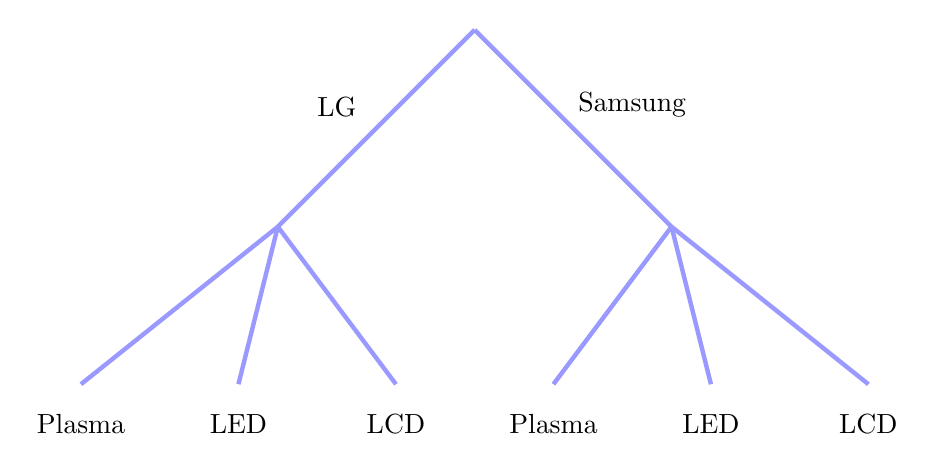
\begin{tikzpicture}
\draw [ultra thick,color=blue!40] (0,2.5) -- (-2.5,0) node[midway, above, xshift=-0.5cm, color=black] {LG};
\draw [ultra thick,color=blue!40] (-2.5,0) -- (-5,-2);
\draw [ultra thick,color=blue!40] (-2.5,0) -- (-3,-2);
\draw [ultra thick,color=blue!40] (-2.5,0) -- (-1,-2);

\draw [ultra thick,color=blue!40] (0,2.5) -- (2.5,0) node[midway, above, xshift=0.75cm, color=black] {Samsung};
\draw [ultra thick,color=blue!40] (2.5,0) -- (5,-2);
\draw [ultra thick,color=blue!40] (2.5,0) -- (3,-2);
\draw [ultra thick,color=blue!40] (2.5,0) -- (1,-2);

\draw [yshift=-2.5cm,xshift=-5cm] node {Plasma};
\draw [yshift=-2.5cm,xshift=-3cm] node {LED};
\draw [yshift=-2.5cm,xshift=-1cm] node {LCD};
\draw [yshift=-2.5cm,xshift=1cm] node {Plasma};
\draw [yshift=-2.5cm,xshift=3cm] node {LED};
\draw [yshift=-2.5cm,xshift=5cm] node {LCD};

\end{tikzpicture}
\end{center}

By counting the number of branches that our decision could follow, it's clear that there are six total possibilities: for each choice of brand, there are three possibilities, so there are \[2 \times 3 = 6 \textrm{ choices}.\]  

Notice that if we switch the order of the decisions, we get the same number of final options:

\begin{center}
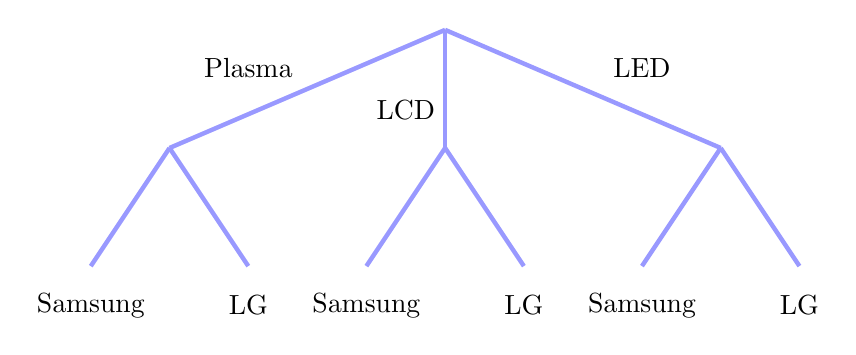
\begin{tikzpicture}
\draw [ultra thick,color=blue!40] (0,1.5) -- (-3.5,0) node[midway, above, xshift=-0.75cm, color=black] {Plasma};
\draw [ultra thick,color=blue!40] (-3.5,0) -- (-4.5,-1.5);
\draw [ultra thick,color=blue!40] (-3.5,0) -- (-2.5,-1.5);

\draw [ultra thick,color=blue!40] (0,1.5) -- (3.5,0) node[midway, above, xshift=0.75cm, color=black] {LED};
\draw [ultra thick,color=blue!40] (3.5,0) -- (4.5,-1.5);
\draw [ultra thick,color=blue!40] (3.5,0) -- (2.5,-1.5);

\draw [ultra thick,color=blue!40] (0,1.5) -- (0,0) node[midway, below, xshift=-0.5cm, color=black] {LCD};
\draw [ultra thick,color=blue!40] (0,0) -- (-1,-1.5);
\draw [ultra thick,color=blue!40] (0,0) -- (1,-1.5);

\draw [yshift=-2cm,xshift=-4.5cm] node {Samsung};
\draw [yshift=-2cm,xshift=-2.5cm] node {LG};
\draw [yshift=-2cm,xshift=-1cm] node {Samsung};
\draw [yshift=-2cm,xshift=1cm] node {LG};
\draw [yshift=-2cm,xshift=2.5cm] node {Samsung};
\draw [yshift=-2cm,xshift=4.5cm] node {LG};

\end{tikzpicture}
\end{center}

We can generalize this to get the \textbf{fundamental counting principle.}

\begin{proc}{Fundamental Counting Principle}
If we are asked to choose one item from each of two separate categories where there are $m$ items in the first category and $n$ items in the second category, then the total number of available choices is \[ m \times n \]
We can generalize this principle to finitely many categories. 
\end{proc}

For instance, if we want to count the number of possible lottery tickets that could be made with numbers that have 4 digits, all we have to do is multiply together the possible values for each digit (note that there are 10 possibilities: 0--9).
\[\underline{10} \cdot \underline{10} \cdot \underline{10} \cdot \underline{10} = 10,000 \textrm{ possible lottery tickets}\]

We are beginning to see the value of such a simple principle for counting; we didn't have to list out all 10,000 possibilities, but we were able to make a quick calculation and know that that's how many there are.

\begin{example}[https://www.youtube.com/watch?v=MhWsP81KJ84]{So much reading!}
There are 21 novels and 18 volumes of poetry on a reading list for a college English course. How many different ways can a student select one novel and one volume of poetry to read during the quarter?

\sol
Since there are 21 choices for which novel to pick and 18 choices for which poetry volume to pick, there are a total of \[\underline{21} \cdot \underline{18} = \boxed{378 \textrm{ choices}}\]
Note that the order in which we make the decision doesn't matter,\\ since $21 \cdot 18 = 18 \cdot 21$.
\end{example}

\begin{try}
Suppose at a particular restaurant you have three choices for an appetizer (soup, salad or bread-sticks), five choices for a main course (hamburger, sandwich, quiche, fajita or pasta) and two choices for dessert (pie or ice cream). If you are allowed to choose exactly one item from each category for your meal, how many different meal options do you have?
\end{try}
\vspace{-0.25in}

\begin{example}[https://www.youtube.com/watch?v=R-yVVNKC0QQ]{Pizza toppings}
Assume you work at a pizza parlor, and you are offering a special on large, two topping pizzas. Your toppings are broken up into two categories:
\begin{center}
\begin{tabular}{l l}
\textbf{Choice of meat} & \textbf{Choice of veggies} \\ \hline
& \\
Pepperoni & Green peppers \\
Sausage & Tomatoes \\
Ham & Onions \\
Grilled chicken & \\ 
\end{tabular} 
\end{center}
The toppings must be chosen with one from each category. How many different two-topping
pizzas can you make?

\sol
Here, there are 4 meat choices and 3 veggie choices, for a total of 
\[\underline{4} \cdot \underline{3} = \boxed{12 \textrm{ choices}}\]
\end{example}

\begin{try}
Assume that you have expanded the special so that you also receive a 2-liter
bottle of soda with your large pizza. Assume your possible drink choices are Pepsi, Diet
Pepsi, Mountain Dew and Root Beer. Now how many different dinner specials can you have,
including pizza and drinks?
\end{try}

We'll do one last example with the fundamental counting principle, but once again, everything boils down to counting the number of possibilities in each category or each stage of the decision-making process.  As long as we can do that, counting the total number of possibilities just involves multiplying those together.
\vfill
\pagebreak

\begin{example}[https://www.youtube.com/watch?v=oSolXixtUy0]{Apartment shopping}
An apartment complex offers apartments with four different choices: the number of bedrooms, number of bathrooms, floor, and view.
\begin{center}
\begin{tabular}{c c c c}
\textbf{Bedrooms} & \textbf{Bathrooms} & \textbf{Floor} & 	\textbf{View} \\ \hline
& & & \\
1 & 1 & first & Lake view \\ 
2 & 2 & second & Golf view \\ 
3 & & & No view\\  
\end{tabular} 
\end{center}
How many apartment options are available?

\sol
Since we are making 4 choices, we'll be multiplying 4 numbers together: the number of options for each choice.
\begin{align*}\underline{3 \textrm{ numbers of bedrooms}} &\times \underline{2 \textrm{ numbers of bathrooms}} \times \underline{2 \textrm{ numbers of floors}}\\ &\times \underline{4 \textrm{ numbers of views}} = \boxed{36 \textrm{ options}}\end{align*}
\end{example}

\begin{try}
You know that you have a multiple choice exam coming up, and you figure
you don't need to study too hard since it is multiple choice. But then you remember the
Fundamental Counting Principle and you decide you better check how many possible ways
there are for you to answer the questions. The exam consists of 10 questions, with each
question having 4 possible choices and only one correct answer per question. If you select
one of these 4 choices for each question and leave nothing blank, how many ways can you
answer the questions? How many ways are there to get a perfect exam?
\end{try}

The fundamental counting principle can even handle questions that sound difficult when they're posed.  For instance, suppose you find yourself in a group of five friends going to a movie.  Two of the five are arguing, and they demand to sit on opposite sides of the row of five seats.  How many ways are there to arrange this group?  Rather than trying to list all the possibilities, all we have to think through is how many options there are for who can sit in each seat.
\begin{enumerate}
\item Only one of the two arguing friends can sit in the first seat, so this seat has two options.
\item One person has sat down, leaving four standing.  The other arguing member, though, cannot sit in the second seat, leaving three options for it.
\item Of the three still standing after the first two seats are filled, only two can sit in the third seat.
\item There's therefore only one option for the fourth seat.
\item Finally, the fifth seat only has one option as well: the other warring member.
\end{enumerate}
Thus there are a total of \[\underline{2} \cdot \underline{3} \cdot \underline{2} \cdot \underline{1} \cdot \underline{1} = 12 \textrm{ possibilities}\]

\subsection{Factorials!}
In many of the examples that we'll see next, it will be convenient to have notation for what we call \textbf{factorials}.  To see this, consider the following example: you want to know how many ways there are to arrange your seven textbooks on the shelf in seven positions.  Following the pattern of the example with the friends sitting at the movie theater, we can see that there are 7 options for the first position, 6 options for the second position (since one has already been placed), 5 options for the third position, and so on.  There are a total of 
\[\underline{7} \cdot \underline{6} \cdot \underline{5} \cdot \underline{4} \cdot \underline{3} \cdot \underline{2} \cdot \underline{1} = 5040 \textrm{ arrangements}\]

Any time we start arranging things in order, we'll see a descending product like this one, so for simplicity's sake, we define that as a factorial (so that we can more easily tell our calculators to calculate it, for instance, and so that our formulas are more concise).

The notation we use is the exclamation mark, so ``7 factorial'' would be written 7!:
\[7! = 7 \cdot 6 \cdot 5 \cdot 4 \cdot 3 \cdot 2 \cdot 1\]

\begin{formula}{Factorials}
The \textbf{factorial} of any positive integer $n$ is defined as the product of every integer from $n$ down to 1:
\[n! = n \cdot (n-1) \cdot (n-2) \cdots (3) \cdot (2) \cdot (1)\]

By definition, $0! = 1$.
\end{formula}

\begin{example}[https://www.youtube.com/watch?v=TIen8pZiUZg]{Movie marathon}
You have been given the job of scheduling the movies for the FCC Movie
Marathon. You have 4 choices for movies: one action movie, one comedy, one drama, and one horror. Luckily
for you, you know the Fundamental Counting Principle. How many different ways are there
to order these 4 movies?

\sol
There are 4 ways to pick the first movie, then 3 ways to pick the second, 2 ways to pick the third, and only 1 way to pick the fourth.  Now we have factorial notation for this:
\[4! = 4 \cdot 3 \cdot 2 \cdot 1 = \boxed{24 \textrm{ possibilities}}\]
\end{example}

\begin{try}
Going back to the movie marathon, since you know that most people don't
like Horror movies you decide that it should go last. With this in mind, how many different
ways is there to arrange the movie marathon?
\end{try}

\subsection{Permutations}
Permutations arise whenever we want to arrange items in order, like in the example of arranging seven textbooks on a shelf.  Not only that, but we can also calculate the number of ways to select, for instance, seven textbooks out of a pool of ten and \emph{then} arrange them in order.\\

Let's think about that example: since we're arranging seven books, there are seven slots to fill.  In the first slot, we have 10 options (the full list of books available), then 9 in the next slot, and so on:
\[\underline{10} \cdot \underline{9} \cdot \underline{8} \cdot \underline{7} \cdot \underline{6} \cdot \underline{5} \cdot \underline{4}\]

Notice how this looks like a factorial calculation, $10!$, but it has been cut off early.  We could always calculate permutations using this same approach, but that cut-off factorial gives us an idea for a shortcut: notice that if we started with $10!$, then divided by $3!$, that would cut off the tail of the factorial after the 4:
\[\dfrac{10!}{3!} = \dfrac{\underline{10} \cdot \underline{9} \cdot \underline{8} \cdot \underline{7} \cdot \underline{6} \cdot \underline{5} \cdot \underline{4} \cdot \cancel{\underline{3} \cdot \underline{2} \cdot \underline{1}}}{\cancel{\underline{3} \cdot \underline{2} \cdot \underline{1}}} = \underline{10} \cdot \underline{9} \cdot \underline{8} \cdot \underline{7} \cdot \underline{6} \cdot \underline{5} \cdot \underline{4}\]

Essentially, to find the number of ways to choose 7 and arrange them, we divide the number of ways to arrange the 10 (10!) by the number of ways to arrange the 3 leftovers (3!).  This is how we calculate permutations, so the number of ways to select 7 textbooks out of 10 and arrange them is
\[\dfrac{10!}{3!}\]

Notice that the 10 is the size of the pool that we can choose from, and the 3 is the number of leftovers, the difference between the total number of available options and the number that we chose.
\pagebreak

\begin{formula}{Permutations}
We say that there are $nPr$ permutations of size $r$ that may be selected from among $n$ choices without replacement when \textbf{order matters}. To compute the number of permutations of $r$ items from a collection of $n$ items, we use the formula below:
\[  nPr = \frac{n!}{(n-r)!}\]
\end{formula}

To simplify the process, we can use a calculator to solve problems like this; many have the permutation formula built in.\\

\begin{proc}{Using Your Calculator}
There are two ways to use your calculator to solve problems involving permutations (and later, combinations): enter the formula with the factorials, or use the built-in permutation function.  Both are found by pressing the \calcbutton{MATH} button and scrolling over to the \texttt{PRB} (probability) menu.

\begin{center}
\begin{tabular}{c c}
\includegraphics[height=0.9in]{CalcFactorial} & \hspace{0.75in} \includegraphics[height=0.9in]{CalcPerm}
\end{tabular}
\end{center}

Note that to use the \texttt{nPr} option, type in the value of $n$ first, then select \texttt{nPr}, then enter the value of $r$ and press \calcbutton{ENTER}.
\end{proc}

\begin{example}[https://www.youtube.com/watch?v=vnvlFNwFUQc]{Arranging CD's}
You have 18 CDs, and you need to arrange 8 of your favorites on the shelf near your stereo.
How many ways can you arrange the CDs, assuming that the order of the CDs makes a
difference to you?

\sol
Using the formula for permutations, $n$ here is 18 (the number that we can choose from) and $r$ is 8 (the number that we are selecting to organize):
\begin{align*}
nPr &= \dfrac{18!}{(18-8)!}\\
&= \dfrac{18!}{10!}\\
&= \boxed{1,764,322,560 \textrm{ possibilities}}
\end{align*}
\end{example}

\begin{try}
How many arrangements can be made using four of the letters of the statement
MATH RULES if no letter is to be used more than once and the space is not considered? (For this we don't care if it
actually makes a word, so ``AUET'' would be one of those 4 letter permutations.)
\end{try}

In case you weren't convinced before, hopefully you agree now that these counting principles are useful, because if you had to list all 1,764,322,560 options in order to count them, you could list one every second and still spend almost 56 years doing so.  Instead, we were able to apply a counting principle and get that result by having our calculator do the arithmetic for us.
\pagebreak

\begin{example}[https://www.youtube.com/watch?v=XGwosYiNY2I]{FCC Math Club}
The math club has 18 members. According to the bylaws they need to have a president,
vice-president and secretary. How many different ways can those positions be filled?

\sol Here, $n$ is 18 and $r$ is 3.  Using the formula: \[nPr = \dfrac{18!}{15!} = \boxed{4896 \textrm{ possibilities}}\]
\end{example}

\begin{try}
Your iPod contains 954 songs and you want the iPod to pick 5 songs at random.
Assuming songs cannot be repeated, how many 5 song play lists can your iPod generate?
\end{try}

Notice that if $n$ and $r$ are the same, like when we arranged 7 textbooks in 7 positions, the formula becomes \[\dfrac{7!}{0!}\] and that should be equal to $7!$, so $0!$ is defined to be equal to 1.\marginnote{Note: $0!=1$}


\subsection{Combinations}
So far we've considered the situation where we chose $r$ items out of $n$ possibilities without replacement and where the order of selection was important. We now focus on a similar situation in which the order of selection is not important.

\begin{example}{Combinations}
A charity benefit is attended by 25 people at which three \$50 gift certificates are given away as door prizes. Assuming no person receives more than one prize, how many different ways can the gift certificates be awarded?

\sol
Using the Basic Counting Rule, there are 25 choices for the first person, 24 remaining choices for the second person and 23 for the third, so there are $25 \cdot 24 \cdot 23 = 13,800$ ways to choose three people. Suppose for a moment that Abe is chosen first, Bea second and Cindy third; this is one of the 13,800 possible outcomes. Another way to award the prizes would be to choose Abe first, Cindy second and Bea third; this is another of the 13,800 possible outcomes.\\

But either way Abe, Bea and Cindy each get \$50, so it doesn't really matter the order in which we select them. In how many different orders can Abe, Bea and Cindy be selected? It turns out there are 6:
\[  ABC \hspace{.3in} ACB \hspace{.3in} BAC \hspace{.3in}  BCA \hspace{.3in} CAB \hspace{.3in}CBA \]
How can we be sure that we have counted them all? We are really just choosing 3 people out of 3, so there are $3 \cdot 2 \cdot 1 = 6$ ways to do this; we didn't really need to list them all; we can just use permutations!\\

So, out of the 13,800 ways to select 3 people out of 25, six of them involve Abe, Bea and Cindy. The same argument works for any other group of three people (say Abe, Bea and David or Frank, Gloria and Hildy) so each three-person group is counted six times. Thus the 13,800 figure is six times too big. The number of distinct three-person groups will be
\[\dfrac{13,800}{6} = \boxed{2300 \textrm{ groups}}\]
\end{example}

It turns out that we can generalize this rule, and if order doesn't matter, we can count the number of ways to choose $r$ items out of $n$ by counting the number of permutations (where order matters) and dividing by $r!$ (the number of ways to arrange the items we've chosen).

\begin{formula}{Combinations}
We say that there are $nCr$ combinations of size $r$ that may be selected from among $n$ choices without replacement when \textbf{order does not matter}. To compute the number of combinations of $r$ items from a collection of $n$ items, we use the formula below:
\[  nCr = \frac{n!}{(n-r)!r!}\]
\end{formula}

Thus, the only distinction between \emph{permutations} and \emph{combinations} is whether or not order matters.  In questions that don't explicitly state whether to use the permutation or combination formula, all we have to consider is whether or not order is important in that scenario.  For instance, when picking a president, vice president, and secretary for a club, order matters, but when picking a committee without ranks, order doesn't matter; all that matters is who got chosen.

\begin{example}[https://www.youtube.com/watch?v=ybwqsaiFgA8]{Student council}
A group of four students is to be chosen from a 35-member class to represent the class on the student council. How many ways can this be done?

\sol
Simply use the combination formula with $n=35$ and $r=4$:
\[nCr = \dfrac{35!}{31! \ 4!} = \boxed{52,360 \textrm{ ways}}\]
\end{example}

\begin{try}
The United States Senate Appropriations Committee consists of 29 members; the Defense Subcommittee of the Appropriations Committee consists of 19 members. Disregarding party affiliation or any special seats on the Subcommittee, how many different 19-member subcommittees may be chosen from among the 29 Senators on the Appropriations Committee?
\end{try}

\begin{proc}{Using Your Calculator}
Combinations can also be calculated using a graphing calculator.  To do so, select the \verb|nCr| operation from the \verb|PRB| (probability) menu.

\begin{center}
\begin{tabular}{c c}
\includegraphics[height=1.25in]{nCr} & \hspace{0.5in} \includegraphics[height=1.25in]{nCr2}
\end{tabular}
\end{center}
\end{proc}

We'll show two more examples, but each of these is simply a matter of applying the correct formula in the right way.\\

Again, to distinguish between permutations (\texttt{nPr}) and combinations (\texttt{nCr}), simply ask, ``is order significant in this problem?''  If it is, that's a permutation, and if not, it is a combination.
\vfill
\pagebreak

\begin{example}[https://www.youtube.com/watch?v=KQVo1KwtF1c]{Quidditch players}
How many different ways can Harry Potter choose 3 players to be ``Chasers''
from a choice of 10 players?

\sol
Does the order of choice matter?  Since all 3 players will fill the same position, there's no difference in what order they are selected, so this is a combination problem:
\[10\ nCr\ 3 = \dfrac{10!}{7! \ 3!} = \boxed{120 \textrm{ ways}}\]
\end{example}

\begin{try}
How many different four-card hands can be dealt from a deck that has 16
different cards?
\end{try}

\begin{example}[https://www.youtube.com/watch?v=LnFSPX3VKXM]{Attending a workshop}
How many different ways can a director select 4 actors from a group of 20
actors to attend a workshop on performing in rock musicals?

\sol
Does the order matter?  No, there is no mention of any distinction based on what order the actors are selected; all that matters is which ones were chosen or not chosen.  Thus, this too is a combination problem.
\[20\ nCr\ 4 = \dfrac{20!}{16! \ 4!} = \boxed{4845 \textrm{ ways}}\]
\end{example}

\begin{try}
You volunteer to pet-sit for your friend who has seven different animals. You
offer to take three of the seven. How many different sets of pets can you care for?
\end{try}

\subsection{Probability and the Counting Methods}
We can use permutations and combinations to help us answer more complex probability questions than we could before, specifically by allowing us to more efficiently count the number of possible outcomes in our sample space and those that correspond to our event.

\begin{example}[https://www.youtube.com/watch?v=d0PaAz2Ro4k]{Bic Pens}
Bic Pens make pens in 4 colors--blue, black, red and green--with 3 tip styles: extra fine, fine and medium. What is the probability of picking one pen at random and having
it be a black pen?

\sol
For this example, we just need the fundamental counting principle; since there are 4 colors and 3 tips, there are a total of 12 pen styles.\\

If we consider black pens, we have 1 color and 3 tips, so there are 3 choices for black pens.\\

Therefore the probability of picking one pen at random and having
it be black is:
\[P(\mbox{black pen}) = \boxed{\frac{3}{12} = \frac{1}{4}}\]
\end{example}

\begin{example}[https://www.youtube.com/watch?v=qJExejyTNzY]{Lottery}

In a certain state's lottery, 48 balls numbered 1 through 48 are placed in a machine and six of them are drawn at random, without replacement. If the six numbers drawn match the numbers that a player had chosen, the player wins \$1,000,000. In this lottery, the order in which the numbers are drawn doesn't matter. Compute the probability that you win the million-dollar prize if you purchase a single lottery ticket.

\sol
Here, we'll use what we know about combinations, since we're picking 6 numbers out of 48 without worrying about the order in which they're arranged.\\

There are \[nCr = \dfrac{48!}{42! \ 6!} = 12,271,512\] ways to choose six numbers, and only one winning combination, so the probability of winning is \[\boxed{\dfrac{1}{12,271,512} \approx 0.00000008}\]
\end{example}

\begin{try}
Suppose you play the Daily Pick 3 everyday, in which three numbers are chosen without replacement, and choose the numbers 214.
You play \$1 straight and \$1 boxed. (Straight means you pick three numbers and in order to
win, you must have those three numbers in the exact same order. Boxed means you win with
any permutation of those three numbers.) What is the probability of you winning the Daily
Pick 3 straight? What is the probability of you winning the Daily Pick 3 boxed?
\end{try}

\begin{example}[https://www.youtube.com/watch?v=D_HPDTJlKNY]{PIN}
A 4-digit PIN is selected. What is the probability that there are no repeated digits?

\sol
There are a total of \[\underline{10} \cdot 
\underline{10} \cdot \underline{10} \cdot \underline{10} = 10,000\] possible PINs, so all we need to find is how many of them have no repeating digits.\\

This is equivalent to choosing 4 digits out of the 10 possible digits (so that we get a distinct value in each of the 4 positions), regardless of order, meaning that there are \[nCr = \dfrac{10!}{6! \ 4!} = 210\] possible PIN codes with no repeating digits.  The probability of this occurring, then, is \[\boxed{\dfrac{210}{10,000} = 0.021}\]
\end{example}

The principle is simple: count the number of total possibilities and count how many ways your event can occur, then divide these two.  In practice, though, it can be tricky to accomplish this counting.  Let's go back to a deck of cards for another example.
\pagebreak

\begin{example}[https://www.youtube.com/watch?v=QXyNszl3_h0]{Drawing cards}
Compute the probability of randomly drawing five cards from a deck without replacement and getting exactly one Ace.

\sol
Getting \textit{exactly} one Ace means getting one Ace and four cards that are not Aces (this seems obvious, but stating it is helpful in order to see the next step): we need to find the number of ways to pick one Ace and the number of ways to pick 4 non-Aces, and then multiply them (remember the fundamental counting principle).  Note that order doesn't matter, so we'll use the \textit{combination} formula.
\begin{align*}
&\textrm{ways to pick one ace } \times \textrm{ ways to pick 4 non-aces}\\
&= _4C_1 \times \ _{48}C_4\\
&= 4 \times 194,580 = 778,320
\end{align*}

Now, to compute the probability of this occurring, we need to divide the number of ways it could happen by the total number of possible hands: $_{52}C_5 = 2,598,960$
\[\boxed{\dfrac{778,320}{2,598,960} \approx 0.2995}\]
\end{example}

\begin{try}
Compute the probability of randomly drawing five cards from a deck of cards and getting three Aces and two Kings.
\end{try}

\begin{example}[https://www.youtube.com/watch?v=vG46K6Fr8Yw]{Movie Order}
Assume that you are still in charge of the FCC movie marathon. Recall the
four types of movies you were planning on showing are Action, Comedy, Drama and Horror.
Assume someone also brought a Thriller to be included in the marathon. In order to find
out the order of the movies, you decide to throw all the names in a hat and plan to draw one
name out of the hat at a time. The order will be determined by how they are pulled out of
the hat. What is the probability of the Thriller being played 4th and the Horror movie being
played 5th?

\sol
\begin{enumerate}
\item How many ways can this scenario happen?

We can do this two ways: using permutations or thinking through the fundamental counting principle; since the order of the fourth and fifth movies is given, all that remains to be ordered is the first three.
\begin{enumerate}
\item Using permutations: $_3P_3 = 6$
\item Using the fundamental counting principle:
\[\underline{3} \cdot \underline{2} \cdot \underline{1} \cdot \underline{1} \cdot \underline{1} = 6\]
\end{enumerate}

\item How many options are there for the order of the movies?

There are 5 movies being organized in 5 slots: \[_5P_5 = 120\]

\item What is the probability of this scenario?

The probability is simply the number of ways the scenario could occur divided by the number of total possibilities:
\[\boxed{\dfrac{6}{120} = 0.05}\]
\end{enumerate}
\end{example}